\documentclass [a4paper,normaltoc,normalfigtabnum, header, espacoumemeio, capchap, capsec, cappre, 12pt,notimes]{abntpoli}

\usepackage[usenames,dvipsnames]{color}
\usepackage{graphicx}
\usepackage{pstricks}
\usepackage{acronym}
\usepackage[brazil]{babel}
\usepackage[T1]{fontenc}
\usepackage{amsmath}
\usepackage{amssymb}
\usepackage{listings}
\usepackage{tocbibind}
\usepackage[labelsep=endash, font=footnotesize]{caption}
\usepackage[alf, abnt-emphasize=bf]{abntcite}
\usepackage[final]{listofsymbols}
\usepackage{url}
\usepackage{textcomp}
\usepackage{imakeidx}
\usepackage{subfig}
\usepackage[section]{placeins}
\usepackage{etoolbox}
\usepackage{dsfont} % fontes matem�ticas duplas como N, Z, R, para designar conjuntos
\usepackage[subfigure]{tocloft}
\usepackage[final]{pdfpages}

%\usepackage{cite}


\renewcommand{\familydefault}{\sfdefault}

\makeindex[title=�ndice]

%muda o comando \bordermatrix para fazer com colchetes
\let\bbordermatrix\bordermatrix
\patchcmd{\bbordermatrix}{8.75}{4.75}{}{}
\patchcmd{\bbordermatrix}{\left(}{\left[}{}{}
\patchcmd{\bbordermatrix}{\right)}{\right]}{}{}

\renewcommand{\ABNTchapterfont}{\bfseries\normalsize\selectfont}
\renewcommand{\ABNTanapsize}{\normalsize}
\renewcommand{\ABNTsectionfontsize}{\normalsize}
\renewcommand{\ABNTsectionfont}{\upshape}
\renewcommand{\ABNTsubsectionfontsize}{\normalsize}
\renewcommand{\ABNTsubsectionfont}{\bfseries}
\renewcommand{\sin}{\operatorname{sen}}
\renewcommand{\arcsin}{\operatorname{arcsen}}
\newcommand{\diag}{\mathop{\mathrm{diag}}}
% 

%\renewcommand{\cftfigfont}{Figura }
%\renewcommand{\cfttabfont}{Tabela }
\setcounter{lofdepth}{1}
\setcounter{tocdepth}{3}
\setcounter{secnumdepth}{3}

\newlength\tablelen
\settowidth\tablelen{\tablename\;}
\addtolength\cfttabnumwidth{\tablelen}
\renewcommand\cfttabpresnum{\tablename\;}
\renewcommand\cfttabaftersnum{\,--\;}

\newlength\figlen
\settowidth\figlen{\figurename\;}
\addtolength\cftfignumwidth{\figlen}
\renewcommand\cftfigpresnum{\figurename\;}
\renewcommand\cftfigaftersnum{\,--\;}


\graphicspath{{./figuras/}}

\allowdisplaybreaks

% Pacote: listings
% Carrega informa��es de suporte �s linguagens. Deixa a linguagem C
% como padr�o e os coment�rios em fonte pequena.
\lstloadlanguages{C}
\lstset{emph={Sum,N},emphstyle=\color{blue},emph=[2]I,emphstyle=[2]\underbar,
   commentstyle=\scriptsize, basicstyle=\scriptsize, language=Matlab,numbers=none,numberstyle=\tiny,
   stepnumber=1,numbersep=5pt,breaklines=true,breakindent=0pt,
   prebreak=\mbox{\tiny$\hdots$},
   postbreak=\mbox{{\color{blue}\tiny$\hdots$}},
   backgroundcolor=\color{gray!10}}
   
   %\lhead{\thechapter}
   
   

\begin{document}
	\pagenumbering{roman}
	
	
\autor{Nome do Autor}
\titulo{T�tulo da Tese}
\orientador{Nome do Orientador}
\local{S�o Paulo}
\areadeconcentracao{Sistemas Eletr�nicos}
\comentario{Tese apresentada � Escola Polit�cnica da \mbox{Universidade} de S�o Paulo para a obten��o do t�tulo de Doutor em Ci�ncias}
\data{Ano}
\capa
\folhaderosto




	\pretextualchapter{Agradecimentos}

Primeiramente, agrade�o ao Prof. ....

Aos colegas ...

Aos meus pais ....

....

Por fim, � quem me financiou.
	
	%\newpage
	\begin{resumo}
   Esta Tese/Disserta��o � sobre....
   Deve conter no m�ximo 500 palavras.
   
   \noindent
   {\bf Palavras-chave}: Palavra-chave 1. Palavra-chave 2. Palavra-chave 3. Palavra-chave 4. Palavra-chave 5. 
 \end{resumo}

\begin{abstract}

\textbf{Thesis title in English}\\

   This Thesis is about....
   It should have maximally 500 words.
   
   \noindent
   {\bf Keywords}: Keyword 1. Keyword 2. Keyword 3. Keyword 4. Keyword 5.
\end{abstract}


	
%	\renewcommand\listfigurename{Lista de Figuras}
	
	\listadefiguras
	\listadetabelas
%	%%% modifica a maneira de apresentar a lista de siglas
	\def\bflabel#1{{{\textsf{#1}}\hfill}}
	\renewenvironment{AC@deflist}[1]%
	      {\if AC@nolist%
		\else%
		    \raggedright\begin{list}{}%
		    {\settowidth{\labelwidth}{\textsf{#1}+8pt}%
		    \setlength{\leftmargin}{\labelwidth}%
		    \setlength{\itemsep}{0.5pt}%
		    \addtolength{\leftmargin}{\labelsep}%
		    \renewcommand{\makelabel}{\bflabel}}%
		 \fi}%
		{\if AC@nolist%
		  \else%
		    \end{list}%
		\fi}%

\pretextualchapter{Lista de Siglas}

\begin{acronym}[NARMAX]
	\acro{USP}[USP]{Universidade de S�o Paulo}
\end{acronym}




	\renewcommand\symheadingname{Lista de S�mbolos}
\renewcommand\symheading{\pretextualchapter{Lista de S�mbolos}}

\opensymdef
	\newsym[S�mbolo 1]{A}{\alpha}
	\newsym[S�mbolo 2]{X}{x}	
\closesymdef


	\listofsymbols	
	%\lhead{\thechapter}
	
	%%% modifica a maneira de apresentar a lista de siglas
	\def\bflabel#1{{{\textsf{#1}}\hfill}}
	\renewenvironment{AC@deflist}[1]%
	      {\if AC@nolist%
		\else%
		    \raggedright\begin{list}{}%
		    {\settowidth{\labelwidth}{\textsf{#1}+8pt}%
		    \setlength{\leftmargin}{\labelwidth}%
		    \setlength{\itemsep}{0.5pt}%
		    \addtolength{\leftmargin}{\labelsep}%
		    \renewcommand{\makelabel}{\bflabel}}%
		 \fi}%
		{\if AC@nolist%
		  \else%
		    \end{list}%
		\fi}%

\pretextualchapter{Lista de Siglas}

\begin{acronym}[NARMAX]
	\acro{USP}[USP]{Universidade de S�o Paulo}
\end{acronym}




	
	\sumario	
	
	%\pagestyle{fancyplain}
	\chapter{Introdu��o}
\label{cap:intro}

\index{problema}
O problema que esta tese aborda .... ~\cite{Kandel2013,Fuglevand1993, Harris1998}. 

Algo importante a saber ao escrever em portugu�s � que os arquivos .tex devem ser salvos com decodifica��o ISO 8859-15.

... \cite{Heckman2012}. 

\section{Objetivos}
\index{objetivos}
\index{exemplo! sigla}
O objetivo central do trabalho apresentado, realizado na \ac{USP} (este foi um exemplo de uso de sigla),  � ...


\section{Estrutura do texto}

\index{estrutura}
Este texto est� organizado da seguinte maneira ... 




		
 	\chapter{Metodologia}
\label{cap:ident}



\index{exemplo de figura}
Exemplo de figura na Fig.~\ref{fig:exemploFig}.
\begin{figure}[ht!]
	\center
	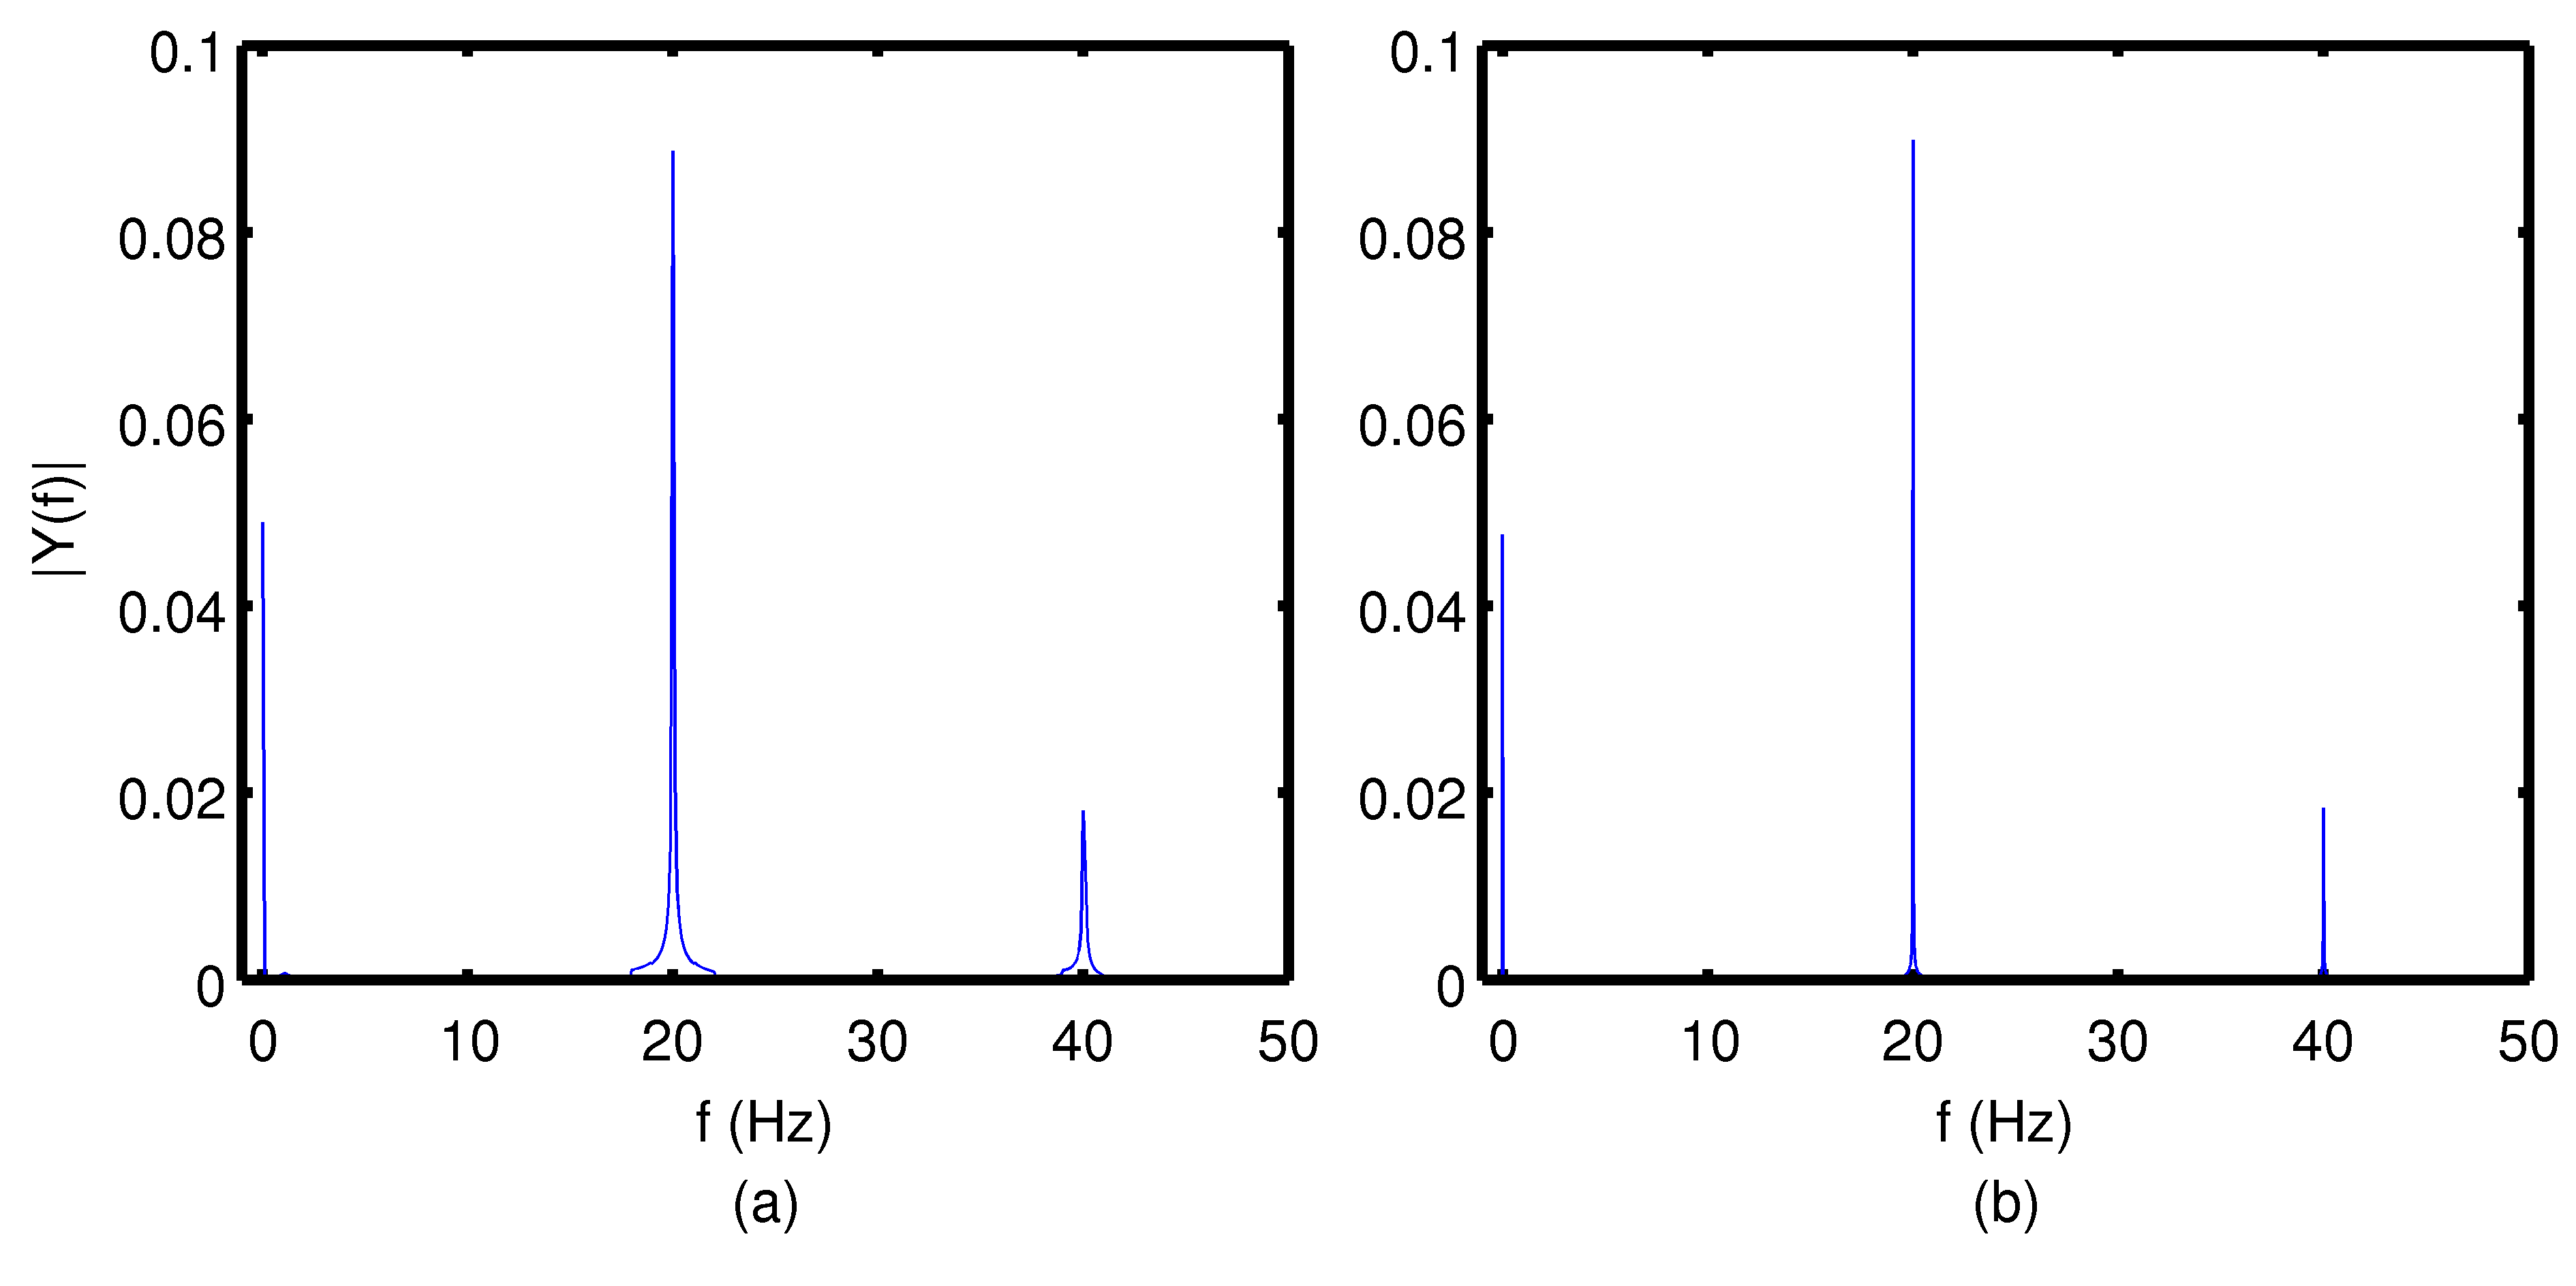
\includegraphics[scale=0.6]{NOFRFExample.png}
	\caption{Exemplo de Figura.}
	\label{fig:exemploFig}
\end{figure}


\index{Exemplo de equa��o}
Exemplo de Equa��o na equa��o~\eqref{eq:exemplo}:
\begin{equation}
  \A = \X + 2
  \label{eq:exemplo}
\end{equation}
 


\section{Mostrando Algoritmo}


\index{Exemplo de algoritmo}
\begin{figure}[!h]
\lstset{keywords=[ 12 ]{func1, indice, naoPertence, para, tamanho, maximo, de, a, se, devolve, soma, e},linewidth=0.95\linewidth,literate={:=}{{$\gets$}}1 {<=}{{$\leqslant$}}1 {>=}{{$\geqslant$}}1 {<>}{{$\neq$}}1 {rho}{{$\rho$}}1   {ws}{{$ws$}}1 {w}{{$w$}}1 {gs_m}{{$gs_m$}}1 {^T}{{$^T$}}1 {^2}{{$^2$}}1 {_s}{{$_s$}}1 {theta}{{$\beta$}}1 {pmatrix}{{\ref{eq:pmatrix}}}1 {^-1}{{$^{-1}$}}1}

\begin{center}
\begin{lstlisting}[frame=single]
func1(param1, param2){
	x := 0
	para (i de 1 a 10){
		x := x + param1 + param2;
	}
	devolve x;	
}
\end{lstlisting}
\end{center}
\vspace{-1.3em}
\caption[Exemplo de Algoritmo]{Exemplo de Algoritmo.}
\label{fig:frols}
\end{figure}

% A matriz $p$, mostrada na Equa��o~\eqref{eq:pmatrix}, quando o modelo segue a representa��o polinomial (Equa��o~\eqref{eq:narmaxpolmodel}), pode ser montada usando o algoritmo na Figura~\ref{fig:pmatrizbuild}. Apesar de parecer simples a montagem desta matriz, achar uma forma geral para o algoritmo n�o foi trivial.  
%

Um exemplo de Tabela � mostrado na Tabela~\ref{tab:exemploTabela}.

\index{Exemplo de Tabela}
\begin{table}[ht!]
\caption{Exemplo de Tabela}
\label{tab:exemploTabela}
\centering
   \begin{tabular}{lrrr}\hline 
	A&B&C&D \\ \hline 
	y(k-1)&2.59e+00&2.44e+00&2.28e+00  \\ 
	y(k-2)&-2.35e+00&-2.12e+00&-1.79e+00  \\ 	
	\hline
    \end{tabular}
\end{table}   






	
	\chapter{Considera��es Finais}
\label{cap:conclusao}

Concluindo, esta Tese/Disserta��o apresentou ....


% 
% 

	
	\ProximoForaDoSumario
	\bibliography{library}
	\setboolean{ABNTNextOutOfTOC}{false}
	
	\apendice
	
	%\chapter{Modelo neuromusculoesquel�tico utilizado}
\label{cap:model}

\index{modelo realista}

\index{modelo!neuromusculoesquel�tico}
O modelo neuromusculoesquel�tico utilizado~\cite{Cisi2008, Elias2012, Watanabe2013, Elias2013, Elias2014, Watanabe2015} representa o \acf{TA} (m�sculo da perna respons�vel pela flex�o dorsal) e os tr�s m�sculos do \acf{TS}: \ac{SOL}, \ac{GM} e \ac{GL} (m�sculos da perna respons�veis pela flex�o plantar), juntamente com os seus respectivos n�cleos de unidades motoras e proprioceptores.

Na Figura~\ref{fig:generalstruct} est� um diagrama simplificado com a vis�o geral do modelo neuromusculoesquel�tico utilizado ao longo deste trabalho. 

\begin{figure}[h!]
	\center
	\includegraphics[scale=0.7]{modelStruct.eps}
	\caption[Vis�o geral do modelo neuromusculoesquel�tico biologicamente realista]{Vis�o geral do modelo neuromusculoesquel�tico biologicamente realista utilizado ao longo deste trabalho. $\act(t)$: sinal de ativa��o muscular; $\F(t)$: for�a gerada pelo m�sculo; $\angvar(t)$: �ngulo de varia��o do tornozelo; $\Lm^M(t)$:comprimento muscular; $\vm(t)$: velocidade de varia��o do comprimento muscular; $\Lm^{MT}(t)$: comprimento do sistema musculotend�neo.}
	\label{fig:generalstruct}
\end{figure}

Cada um dos m�sculos que comp�e o modelo da Figura~\ref{fig:generalstruct} � modelado separadamente. Desta forma, cada um dos m�sculos tem os sinais $\act(t)$, $\F(t)$, $\Lm^M(t)$, $\vm(t)$ e $\Lm^{MT}(t)$ calculados de forma independente dos outros m�sculos. 

Nas se��es a seguir, cada um dos blocos da Figura~\ref{fig:generalstruct} � explicado de forma detalhada.

\section{Modelo do n�cleo de unidades motoras}
\label{sec:pool}

\index{modelo!n�cleo de unidades motoras}
O modelo do n�cleo de unidades motoras usado foi descrito em~\cite{Cisi2008, Elias2012, Watanabe2013,Elias2014}. Na Figura~\ref{fig:poolstruct} est� um diagrama da estrutura do modelo do n�cleo de unidades motoras. 


\begin{figure}[ht!]
	\center
	\includegraphics[scale=0.7]{poolStruct_PTTSTA.eps}
	\caption[Estrutura do modelo de n�cleo de unidades motoras]{Estrutura do n�cleo de unidades motoras usado nesse estudo (a) vis�o esquem�tica do tibial anterior (TA). O n�cleo de unidades motoras do TA consiste em seus motoneur�nios (MNs) e suas respectivas unidades musculares (UM). $\act_{\text{TA}}$: sinal de ativa��o do TA; (b) vis�o esquem�tica do tr�ceps sural (TS) e seus tr�s m�sculos: S�leo (SOL), Gastrocn�mio Medial (GM) e Gastrocn�mio Lateral (GL). O n�cleo de unidades motoras de cada m�sculo do TS consiste em seus MNs e suas respectivas UMs. $\act_{\text{SOL}}, \act_{\text{GM}}, \act_{\text{GL}}$: sinal de ativa��o do SOL, GM e GL, respectivamente; (c) representa��o esquem�tica das unidades motoras (MNs e UMs) de um m�sculo. Cada um dos N processos pontuais de renova��o representando os ax�nios descendentes e provindos dos diferentes proprioceptores (reflexos) se conecta a uma fra��o dos MNs. Cada UM recebe um trem de potenciais de a��o (PAs) do seu MN. Esse trem de PAs � filtrado por um sistema de segunda-ordem criticamente amortecido. Cada um desses sinais filtrados � somado para produzir o sinal de ativa��o $a$; (d)  trem de 
processos pontuais de renova��o representando um trem de PAs de um ax�nio; (e) circuito usado para representar o modelo de MN; $g_{syn_1}$ a $g_{syn_M}$:condut�ncia sin�ptica para sinapse 1 a $M$; $g_c$: condut�ncia de acoplamento; $g_{Ld}$ e $g_{Ls}$: condut�ncia de fuga dendr�tica e do soma, respectivamente; $g_{Na}$, $g_{Kf}$ e $g_{Ks}$: condut�ncias de $\text{Na}^+$, $\text{K}^+$ r�pido e $\text{K}^+$ lento, respectivamente; $E_L$: potencial de Nernst; $E_{Na}$ e $E_K$: potencial de equil�brio de $\text{Na}^+$ e $\text{K}^+$, respectivamente; $E_{syn_1}$ a $E_{syn_M}$: potencial de revers�o das sinapses 1 a $M$; $C_s$ e $C_D$: capacit�ncias som�ticas e dendr�ticas, respectivamente; $V_S$ e $V_D$: potencial de membrana do soma e do dendrito, respectivamente; (f) uma parcela do sinal de ativa��o produzida por uma UM; (g) fun��o de satura��o de uma UM.}
	\label{fig:poolstruct}
\end{figure}

\index{modelo!motoneur�nio}
Os  \acfp{MN}  foram representados por modelos do tipo {\it conductance-based} com dois compartimentos, um representando o soma e outro a arboriza��o dendr�tica do \ac{MN}. O circuito el�trico que representa o comportamento de um \ac{MN} est� na Figura~\ref{fig:poolstruct}(e). A solu��o das equa��es diferenciais de Hodgkin-Huxley dos canais i�nicos~\cite{Hodgkin1952a} s�o aproximadas por pulsos~\cite{Destexhe1997}. Os par�metros dos \acp{MN} s�o distribu�dos linearmente de forma que o princ�pio do tamanho~\cite{Henneman1965b} seja obedecido. Mais detalhes podem ser encontrados em~\citeonline{Cisi2008, Elias2012,Watanabe2013} e \citeonline{Elias2014}.

Para cada \ac{PA} que um \ac{MN} gera, a sua \ac{UM} correspondente gera um sinal que � obtido utilizando um filtro de segunda-ordem criticamente amortecido~\cite{Cisi2008} (ver Figura~\ref{fig:poolstruct}(f)). O sinal gerado por uma \ac{UM} em resposta a um \ac{PA} (resposta ao impulso), chamado de abalo, segue a seguinte equa��o:
\begin{equation}
  a(t)=\frac{t}{\Tp}e^{\left(1-\frac{t}{\Tp}\right)}, t\geqslant0
  \label{eq:twitch}
\end{equation}
em que \Tp � o tempo que o sinal leva para atingir seu valor m�ximo. Os valores de \Tp variam para cada \ac{UM}, de forma que o princ�pio do tamanho seja obedecido~\cite{Henneman1965}. Esses sinais de cada \ac{UM} s�o multiplicados por uma satura��o sigmoidal~\cite{Watanabe2013} (ver Figura~\ref{fig:poolstruct}(g)) e ent�o s�o somados para gerar o sinal de ativa��o $\act(t)$ de cada m�sculo (ver Figura~\ref{fig:poolstruct}(c)). A fun��o de satura��o de cada \ac{UM} foi ajustada de forma que cada \ac{UM} atingisse sua ativa��o tet�nica quando a frequ�ncia de disparos do seu respectivo \ac{MN} atingisse um dado n�vel, de acordo com os dados de~\citeonline{Enoka2001} e para que o valor da amplitude do sinal gerado em resposta a um \ac{PA} tivesse os mesmos valores encontrados em~\citeonline{Garnett1979, Buchthal1980} e \citeonline{Bellemare1983}. Ap�s a satura��o, os sinais obtidos de cada uma das \ac{UM} s�o somados e normalizados pela for�a m�xima de cada um dos m�sculos~\cite{Menegaldo2009}. Cada um dos m�sculos tem um sinal de ativa��o diferente (ver Figura~\ref{fig:poolstruct}(a,b)). O sinal de ativa��o de cada m�sculo � composto de um sinal de ativa��o para as fibras lentas $\act_I(t)$ e outro para as fibras r�pidas $\act_{II}(t)$ (ver se��o~\ref{sec:hill}). O sinal $\act_I(t)$ de cada m�sculo prov�m das unidades motoras de~\ac{S} e o sinal $\act_{II}(t)$ de cada m�sculo prov�m das unidades motoras de~\ac{FR} e \ac{FF}. No caso de simula��es com contra��es isom�tricas, n�o � necess�ria a utiliza��o de modelo de m�sculo. Neste caso a for�a muscular $\F(t)$ � igual ao sinal de ativa��o $\act(t)$ sem a normaliza��o pela for�a m�xima. Na Tabela~\ref{tab:nummu} est� a quantidade de unidades motoras utilizada em cada m�sculo.

\begin{table}[ht!]
\caption[N�mero de unidades motoras do modelo]{N�mero de unidades motoras adotado no modelo para cada m�sculo do TS e do TA divididos por tipo. S: \acl{S}; FR: \acl{FR}; FF:\acl{FF}}
\label{tab:nummu}
\centering
    \begin{tabular}{lccc}
    \hline
     N�cleo motor& tipo S&tipo FR& tipo FF\\
     \hline
     \acf{SOL}&800&50&50\\
     \acf{GM}&300&150&150\\
     \acf{GL}&130&65&65\\
     \acf{TA}&250&50&50\\
     \hline
    \end{tabular}
\end{table}

\index{modelo!condut�ncia sin�ptica}
Um elemento particularmente importante para a realiza��o da identifica��o do modelo � a gera��o da condut�ncia sin�ptica, e por esse motivo essa gera��o ser� explicada mais detalhadamente a seguir. Os valores dos par�metros do modelo da condut�ncia sin�ptica descritos a seguir s�o para os ax�nios do comando descendente (condut�ncia sin�ptica excitat�ria dendr�tica). Os par�metros das demais sinapses podem ser encontrados em~\citeonline{Elias2013c}.

O decurso temporal da condut�ncia sin�ptica no compartimento dendr�tico � descrito pela seguinte equa��o diferencial:
\begin{equation}
  \dot{\recneu}(t) = \alpha\neurotr[1-\recneu(t)] - \beta \recneu(t)
  \label{eq:conddif}
\end{equation}
em que $< \dot{ } >$ representa a derivada em rela��o ao tempo, $\recneu(t)$ representa a fra��o de receptores ligados a neurotransmissores, $\alpha$ e $\beta$ s�o as taxas constantes direta e reversa para a liga��o de neurotransmissores, respectivamente, e $\neurotr$ � a concentra��o de neurotransmissor lan�ado na fenda sin�ptica.

\citeonline{Destexhe1994} consideram que $\neurotr$ � um pulso, j� que essa concentra��o cresce e decresce muito rapidamente. Com essa suposi��o, a Eq.~\eqref{eq:conddif} pode ser resolvida de forma anal�tica. Desta forma, durante o pulso em que $\neurotr=T_{max}$ ($T_{max}=1$ mM), $r(t)$ � dado pela seguinte equa��o:
\begin{equation}
    r(t-t_0) = r_{\infty}+[r(t_0)-r_{\infty}]e^{\left(-\frac{t-t_0}{\tau_r}\right)}, \, t_0\leqslant t<t_1
    \label{eq:condOn}
\end{equation}
com $r_{\infty}=\frac{\alpha T_{max}}{\alpha T_{max}+\beta}$, a constante de tempo $\tau_r=\frac{1}{\alpha T_{max}+\beta}$, $t_0$ � o instante da ocorr�ncia de um \ac{PA} no ax�nio correspondente �quela sinapse e $t_1$ � o instante em que o pulso acaba. Foi adotado $\alpha=0,5\text{ ms}^{-1}$ e $\beta=2,5\text{ ms}^{-1}$. Ap�s o pulso, com $\neurotr=0$~mM, $r(t)$ � dado por:
\begin{equation}
  r(t-t_1)=r(t_1)e^{-\beta(t-t_1)}, \,t\geqslant t_1
   \label{eq:condOff}
\end{equation}

A dura��o do pulso ($t_1-t_0$) foi adotada como 0,2~ms, de forma que a satura��o sin�ptica ocorre para frequ�ncias dos processos dos ax�nios descendentes maiores que 5~kHz. 

A condut�ncia sin�ptica  $g_{\text{syn}_n}$ da sinapse $n$ � dada pelo produto entre $r_n(t)$ e a m�xima condut�ncia sin�ptica ($\bar{g}_{\text{syn}}=600\text{ nS}$). As sinapses do mesmo tipo (neste caso, excitat�rias feitas com os ax�nios descendentes) podem ser somadas em um �nico valor de condut�ncia:
\begin{equation}
  g_{\text{syn}}(t)=\sum\limits_{n=1}^M \bar{g}_{\text{syn}}r_{n} = \sum\limits_{n=1}^M g_{\text{syn}_n}
  \label{eq:condgbar}
\end{equation}

O processo de gera��o da condut�ncia sin�ptica est� esquematizado na Figura~\ref{fig:SynCond}.

\begin{figure}[ht!]
	\center
	\includegraphics[scale=0.7]{SyConductance.eps}
	\caption[Gera��o da condut�ncia sin�ptica]{Gera��o da condut�ncia sin�ptica. Em cada uma das tr�s colunas � direita � mostrado o processo da gera��o da condut�ncia $g_{\text{syn}_n}$ de uma sinapse. (a) concentra��o de neurotransmissor $\neurotr$ lan�ado na fenda sin�ptica. Os instantes em que os pulsos de concentra��o acontecem s�o os mesmos dos {\it spikes} que chegam do ax�nio correspondente �quela sinapse (ver Figura~\ref{fig:poolstruct}(c)). � esquerda em destaque um pulso de \neurotr. (b) Fra��o de receptores ligados a neurotransmissores $r_n(t)$ em cada sinapse. � esquerda em destaque est� o decurso temporal de $r_n(t)$ em resposta � um pulso de \neurotr. (c) condut�ncia sin�ptica $g_{\text{syn}_n}$ de cada sinapse obtida pela multiplica��o de $r_n(t)$ por $\bar{g}$. � esquerda em destaque est� o decurso temporal de $g_{\text{syn}_n}$ relativo a um pulso de \neurotr. (d) condut�ncia sin�ptica \cond do MN obtida pela soma de cada uma das $g_{\text{syn}_n}$}
	\label{fig:SynCond}
\end{figure}

No modelo, o c�lculo da condut�ncia sin�ptica $\cond(t)$ � feito utilizando o algoritmo de~\citeonline{Lytton1996}, que calcula  $\cond(t)$ de forma eficiente. Basicamente, este algoritmo se baseia na linearidade e invari�ncia no tempo do modelo cin�tico aproximado, que descreve a a��o sin�ptica no compartimento dendr�tico (Eq.~\eqref{eq:condOn} e Eq.~\eqref{eq:condOff}). Uma �nica vari�vel � utilizada para representar a superposi��o das ativa��es sin�pticas que chegam em um determinado \ac{MN}.  Ao inv�s de tratar cada ativa��o sin�ptica de forma individual, o algoritmo usa a informa��o de um peso de cada sinapse em cada instante para gerar o valor da condut�ncia $\cond(t)$. Mais detalhes podem ser encontrados em~\citeonline{Lytton1996}. 

\index{modelo!comando descendente}
\index{processo estoc�stico}
Outro elemento do modelo s�o os ax�nios que fazem conex�es sin�pticas com os \acp{MN}, como o comando descendente e os aferentes. Cada um dos $N$ ax�nios geram os disparos de forma independente dos outros ax�nios. A gera��o dos disparos seguem um processo pontual estoc�stico com uma determinada distribui��o, como por exemplo distribui��o Poisson ou gama~\cite{Papoulis1991a}. \index{modelo!conectividade}Cada um dos ax�nios se conecta a uma determinada porcentagem, chamada de conectividade, dos \acp{MN} de forma aleat�ria. Por exemplo, no caso de um ax�nio ter conectividade 30\%  e o n�cleo de \acp{MN} possuir 100 \acp{MN}, este ax�nio se conectar� a aproximadamente 30 \acp{MN}, escolhidos de forma aleat�ria. 


\section{Modelo de m�sculo}
\label{sec:hill}

\index{modelo!m�sculo}
\index{modelo!Hill}

O modelo de m�sculo utilizado foi um modelo tipo Hill, similar ao descrito em~\citeonline{Menegaldo2009}, por�m acrescido de uma massa, para fins de estabilidade num�rica, e de dois elementos contr�teis, um representando as fibras lentas ($\C_I$) e outro representando as fibras r�pidas ($\C_{II}$)~\cite{Chaud2012a, Watanabe2012e}. O sinal de ativa��o $\act_I(t)$ \index{ativa��o, sinal de} � obtido das unidades motoras de fibras de tipo \ac{S}. Da mesma forma, o sinal de ativa��o $\act_{II}(t)$ � obtido das unidades motoras de fibras de tipo \ac{FR} e \ac{FF} do n�cleo de unidades motoras (ver se��o~\ref{sec:pool}). A Figura~\ref{fig:hillModel} cont�m um diagrama do modelo de m�sculo tipo Hill utilizado para cada um dos tr�s m�sculos do \ac{TS} e o \ac{TA}, juntamente com os dois proprioceptores j� implementados no sistema (ver se��o~\ref{sec:proprio}).


\begin{figure}[ht!]
	\center
	\includegraphics[scale=0.7]{hillModel.eps}
	\caption[Modelo de m�sculo tipo Hill]{Modelo de m�sculo tipo Hill, juntamente com os proprioceptores (em azul). $\km^{PE}$: par�metro do elemento el�stico passivo em paralelo; $\Ba$: par�metro do elemento viscoso passivo em paralelo; $\C_{I}$: elemento contr�til das fibras lentas; $\C_{II}$: elemento contr�til das fibras r�pidas; \m: massa muscular; $\km^T$: par�metro do elemento el�stico do tend�o; \angpen: �ngulo de pena��o; $\Lm^M$: comprimento do m�sculo; $\Lm^T$: comprimento do tend�o; $\Lm^{MT}$: comprimento do sistema m�sculotend�neo. $\act_I$: sinal de ativa��o das fibras lentas; $\act_{II}$: sinal de ativa��o das fibras r�pidas; $\freq_{Ia}$: frequ�ncia de disparos dos aferentes Ia; $\freq_{II}$: frequ�ncia de disparos dos aferentes tipo II; $\freq_{Ib}$: frequ�ncia de disparos dos aferentes Ib; MS: \acl{MS}; OTG: \acl{GTO}; $\F^T$: for�a produzida pelo tend�o.}
	\label{fig:hillModel}
\end{figure}

Os elementos $\km^{PE}$ e  \Ba modelam a parte passiva da for�a ($\F^{PE}$) de cada m�sculo. Essa for�a � dada por:
\begin{equation}
    \tilde{\F}^{PE}(t) = \frac{\exp\left[\km^{PE}\left(\frac{\tilde{\Lm}^M(t) - 1}{\strain^M} \right) \right]}{\exp(\km^{PE})} + \Ba \tilde{\vm}(t)
\end{equation}
em que $< \tilde{} >$ representa a grandeza sendo normalizada pelos valores $\F_0$ (for�a muscular m�xima) e $\Lm_0$ (comprimento �timo) da maneira apropriada (os valores de for�a s�o normalizados por $\F_0$, os comprimentos s�o normalizados por $\Lm_0$ e as combina��es desta grandeza s�o normalizados com combina��es de $\F_0$ e $\Lm_0$), e $\strain^M$ � um par�metro relacionado � diferen�a entre  $\Lm^M(t)$ e $\Lm_0$ e � magnitude da for�a produzida pelo elemento el�stico passivo em paralelo. 

A for�a no tend�o � dada por:
\begin{equation}
  \tilde{\F}^T(t)=\km^T c^T \ln\left[\exp\left(\frac{\tilde{\Lm}^T(t)-\Lm_r^T}{c^T} + 1 \right) \right] 
\end{equation}

O comprimento do sistema musculotend�neo $\Lm^{MT}(t)$ (sistema composto pelo m�sculo e o tend�o), o comprimento da fibra muscular $\Lm^M(t)$ e o comprimento do tend�o $\Lm^{T}(t)$  est�o relacionados pela seguinte equa��o:

\index{sistema musculotend�neo}
\index{modelo!a@�ngulo de pena��o}
\begin{equation}
  \Lm^{MT}(t) = \Lm^T(t)+\Lm^M(t)\cos[\angpen(t))]
\end{equation}
em que $\Lm^{MT}(t)$ � obtido do sistema mec�nico (ver se��o~\ref{sec:mec}) e $\angpen(t)$ � o �ngulo de pena��o do m�sculo e � dado por: 
\begin{equation}
 \angpen(t) = \arcsin\left(\frac{\sin(\angpen_0)}{\tilde{\Lm}^M(t)} \right)
\end{equation}
em que $\angpen_0$ � o �ngulo de pena��o inicial.

A for�a gerada pelos elementos contr�teis $\F^C(t)$ �:
\begin{equation}
    \tilde{\F}^C(t) = \act_I(\tempo).\fl_{I}(\tilde{\Lm}^M(t)).\fv_{I}(\tilde{\Lm}^M(t), \tilde{\vm}(t)) + \act_{II}(\tempo).\fl_{II}(\tilde{\Lm}^M(t)).\fv_{II}(\tilde{\Lm}^M(t), \tilde{\vm}(t))
\end{equation}\index{for�a}
em que fl � a curva for�a-comprimento e fv � a curva for�a-velocidade dos elementos contr�teis~\cite{Hill1938}. As curvas for�a-comprimento e for�a-velocidade s�o as mesmas utilizadas em~\citeonline{Cheng2000}. \index{modelo!curva for�a-comprimento}\index{modelo!curva for�a-velocidade}

Tendo os valores calculados anteriormente, a acelera��o da massa \m � calculada usando as leis de Newton. Para obter a velocidade de contra��o muscular $\vm(t)$ a acelera��o da massa \m � integrada uma vez e para obter o comprimento muscular $\Lm^M(t)$ a acelera��o da massa \m � integrada duas vezes:
\begin{equation}
  \dot{\tilde{\vm}}(t) = \frac{\F_0}{\m}\left[\tilde{\F}^T(t)\cos\left(\angpen(t) \right) - \left(\tilde{\F}^C(t) + \tilde{\F}^{PE}(t)\cos^2\left(\angpen(t) \right) \right)\right]
\end{equation}

Na Tabela~\ref{tab:hillparam} est�o todos os par�metros adotados para o modelo tipo Hill  ao longo deste trabalho, obtidos em~\citeonline{Cheng2000, Thelen2003, Arnold2010} e \citeonline{DeVlugt2012}.

\begin{table}[h!]
\caption[Par�metros utilizados no modelo de Hill]{Par�metros utilizados no modelo de Hill~\cite{Cheng2000, Thelen2003, Arnold2010, DeVlugt2012}}
\label{tab:hillparam}
\centering
  \begin{tabular}{llcccc}
  \hline
      Par�metro&Unidade&SOL&GM&GL&TA\\
      \hline
      $\F_0$ &N & 3586&1306&606&674\\
      $\Lm_0$ &cm&4,90&5,70&6,40&6,80\\
      \m &kg & 0,53&0,22&0,12&0,15\\
      $\km^{PE}$ &$\F_0/\Lm_0$&5&5&5&5\\
      \Ba&$\F_0.s/\Lm_0$ &0,005&0,005&0,005&0,005\\
      $\strain^M$&-&0,5&0,5&0,5&0,5\\
      $\angpen_0$&graus&28,3&9,9&12&9,6\\
      $\Lm^T_0$&cm&28,9&42,4&41,3&24,9\\
      $\km^T$&$\F_0/\Lm_0^T$&27,8&27,8&27,8&27,8\\
      $c^T$&-&0,005&0,005&0,005&0,005\\
      $\Lm_r^T$&$\Lm_0^T$&0,96&0,96&0,96&0,96\\
      \hline
  \end{tabular}
\end{table}

\section{Modelo de proprioceptores}
\label{sec:proprio}
\index{modelo!proprioceptores}
Aqui ser�o descritos os dois tipos de proprioceptores implementados no modelo: o \ac{MS} e o \ac{GTO}.  

\index{modelo!fuso muscular}
O modelo de \ac{MS} utilizado � o modelo apresentado por~\citeonline{Mileusnic2006c} e usado em~\citeonline{Chaud2012a}. O  modelo de fuso � colocado em paralelo � fibra muscular (ver Figura~\ref{fig:hillModel}). Ele tem como entrada o comprimento $\Lm^M$ e a varia��o de comprimento muscular $v$ (obtidos do modelo de m�sculo tipo Hill) e retorna a frequ�ncia de disparo m�dia dos aferentes Ia ($\freq_{I_a}$) e dos aferentes do tipo II ($\freq_{II}$). A $\freq_{I_a}$ � uma combina��o do comportamento est�tico e din�mico da fibra muscular. Por outro lado, a $\freq_{II}$ tem informa��o apenas do comportamento est�tico da fibra. Tendo as frequ�ncias $\freq_{I_a}$ e $\freq_{II}$ dos aferentes, s�o gerados os disparos de cada aferente Ia e II. Esses aferentes disparam com uma frequ�ncia m�dia igual a $\freq_{I_a}$ e $\freq_{II}$, respectivamente, com os \acp{ISI} seguindo um processo gama de ordem 25. O valor da ordem dos processos gama dos aferentes Ia e II foi ajustado para que a variabilidade dos disparos dos processos fosse compat�vel com dados experimentais~\cite{Matthews1969}.
\index{ISI}
\index{modelo!o@�rg�o tendinoso de Golgi}
\index{processo estoc�stico!gama}

O modelo de \ac{GTO} � o mesmo reportado por~\citeonline{Lin2002}. A frequ�ncia de disparo $\freq_{I_b}$ � dada por:
\begin{align}
  G(t) =& G_1\ln\left(\frac{\F^T(t)}{G_2} + 1 \right)\\
  \frac{\freq_{I_b}(\freqcomp)}{G(\freqcomp)} =& 40\frac{1,70\freqcomp^2+2,58\freqcomp+0,40}{\freqcomp^2+2,20\freqcomp+0,40}  
\end{align}
em que $G_1$ e $G_2$ s�o constantes iguais a 60~Hz e 4~N, respectivamente e $s$ � a frequ�ncia complexa provinda da transformada de Laplace. Tendo a frequ�ncia $\freq_{I_b}$ dos aferentes Ib, s�o gerados os disparos de cada aferente Ib. Esses aferentes disparam com uma frequ�ncia m�dia igual a $\freq_{I_b}$, com os \acp{ISI} seguindo um processo gama de ordem 30. O valor da ordem dos processos gama dos aferentes Ib foi ajustado para que a variabilidade dos disparos dos processos fosse compat�vel com dados experimentais~\cite{Matthews1969}.

Na Tabela~\ref{tab:affnum} est�o as quantidades de cada tipo de fibra aferente para cada um dos m�sculos considerados no modelo.

\begin{table}[h!]
\caption{Quantidade de fibras aferentes para cada m�sculo}
\label{tab:affnum}
\centering
 \begin{tabular}{lccc}
  \hline
  M�sculo&Ia&II&Ib\\
  \hline
  \acf{SOL}&400&500&300\\
  \acf{GM}&160&200&120\\
  \acf{GL}&160&200&120\\
  \acf{TA}&280&350&140\\
  \hline
 \end{tabular}
\end{table}


\section{Modelo mec�nico}
\label{sec:mec}


 Neste trabalho � utilizado um modelo mec�nico, no qual o sistema neuromuscular pode atuar: um modelo mec�nico representando o tornozelo utilizado para o estudo de \ac{TF} e \ac{TP}. O modelo � de segunda-ordem, linear e invariante no tempo e � apresentado a seguir. Ap�s a apresenta��o do modelo mec�nico, � mostrada a obten��o do comprimento musculotend�neo $\Lm^{MT}$ e do momento de cada m�sculo. 
 
 \subsection{Modelo de tornozelo}
 \label{sec:foot}
 
 \index{modelo!tornozelo}
 \index{tarefa de posi��o}
 \index{tarefa de for�a}
 O modelo mec�nico que representa o tornozelo pode ser utilizado em duas condi��es diferentes: \ac{TF}, em que o �ngulo do tornozelo n�o varia, e \ac{TP}, com o �ngulo do tornozelo variando. Este modelo  foi utilizado  em ~\citeonline{Watanabe2013a, Watanabe2013b}. Na Figura~\ref{fig:foot} est� uma representa��o deste sistema.

\begin{figure}[ht!]
	\center
	\includegraphics[scale=0.3]{foot.eps}
	\caption[Modelo mec�nico do tornozelo]{Modelo mec�nico do tornozelo. $W$: momento provindo de uma carga; $\Mom_p$: momento passivo do tornozelo; $\Mom_g$: momento devido � acelera��o da gravidade; \Mom: momento ativo exercido pelo tornozelo; $d_f$: dist�ncia do centro do p� ao ponto de rota��o do tornozelo; $\theta_l$: �ngulo que a perna faz com o solo; \angvar: �ngulo de varia��o do tornozelo.}
	\label{fig:foot}
\end{figure}

Durante a \ac{TP}, o �ngulo \angvar varia de acordo com:
\begin{equation}
    \ddot{\angvar} = \frac{\Mom - M_g - M_p + W}{\inertia_f}
\end{equation}
em que \Mom � o torque ativo (valores positivos representam dorsoflex�o e valores negativos flex�o plantar), $\Mom_p$ � o torque passivo (devido � viscoelasticidade dos tecidos), $W$ � o momento provindo de uma carga, $\inertia_f$ � o momento de in�rcia do p� e $\Mom_g$ � o torque gravitacional. Obtida a acelera��o angular $\ddot{\angvar}$, integra-se duas vezes esse valor para obter $\dot{\angvar}$ e \angvar. O torque $\Mom_p$ � obtido por:
\index{torque}
\begin{equation}
 \Mom_p= \Ba_A\dot{\angvar}(t) + \km_A\angvar(t) 
\end{equation}
em que $\Ba_A=1,1\text{ N.m.s/rad}$ e $\km_A = 320\text{ N.m/rad}$ s�o a viscosidade e a elasticidade passiva do tornozelo, respectivamente (devido � viscoelasticidade dos tecidos). O $\Mom_g$ � obtido por:
\begin{equation}
    \Mom_g=d_fm_f\grav\sin(\theta_l-\angvar)
\end{equation}
com $d_f = 0,052$ m, representando a dist�ncia entre o centro do p� e o ponto de rota��o do tornozelo, $\grav=9,81 \text{ m/s}^2$ (acelera��o da gravidade), $m_f = 2,01$ kg (massa do p�) e $\theta_l = \pi/4$~rad (�ngulo da perna com o solo).

%  \subsection{Modelo de p�ndulo invertido}
%  \index{modelo!p�ndulo invertido}
% \index{controle postural}
%  O modelo de p�ndulo invertido est� representado na Figura~\ref{fig:invertedPendulum}. Ele foi utilizado em~\citeonline{Elias2013b}.
% 
% \begin{figure}[ht!]
% 	\center
% 	\includegraphics[scale=0.7]{invertedPendulum.eps}
% 	\caption[Modelo mec�nico do p�ndulo invertido]{Modelo mec�nico do p�ndulo invertido utilizado para modelar o controle da postura ereta quieta. $h_B$: altura do centro de massa; $\m_b$: massa corporal; $\grav$: acelera��o da gravidade; $y_G$: dist�ncia do centro de massa em rela��o ao solo; $\Mom$: momento ativo exercido pelo tornozelo; $y_P$: dist�ncia do centro de rota��o do tornozelo ao centro de press�o; $F_R$: for�a de rea��o aplicada pelo solo no centro de press�o; \angvar: �ngulo de varia��o do p�ndulo}
% 	\label{fig:invertedPendulum}
% \end{figure}
% 
% Os valores da massa corporal e altura do centro de massa adotados s�o: $\m_B= 60\text{ kg}$ e $\h_B=0.85\text{ m}$. O �ngulo \angvar varia de acordo com:
% 
% \begin{equation}
% 	  \ddot{\angvar} = \frac{\Mom -\Mom_p + \Mom_g}{\inertia_B}
% \end{equation}
% 
% em que $\inertia_B=(4/3)\m_B\h_B^2$ � o momento de in�rcia do corpo. Obtida a acelera��o angular $\ddot{\angvar}$, integra-se duas vezes esse valor para obter $\dot{\angvar}$ e \angvar. O torque passivo � obtido utilizando:
% 
% \begin{equation}
%  \Mom_p= \Ba_A\dot{\angvar}  + \km_A\angvar
% \end{equation}
% 
% em que $\Ba_A=5,81\text{ N.m.s/rad}$ e $\km_A = 320\text{ N.m/rad}$ s�o a viscosidade e a elasticidade passiva do tornozelo, respectivamente (devido � viscoelasticidade dos tecidos). O torque gravitacional � computado usando:
% 
% \begin{equation}
%   \Mom_g=\m_B\grav\h_B\sin(\angvar)
%   \end{equation}
  
  \subsection{C�lculo do comprimento do sistema m�sculotend�neo e do momento}
  
  
O comprimento do m�sculo-tend�o $\Lm^{MT}$ e o bra�o-de-momento \Rm, utilizados nos dois modelos mec�nicos (tornozelo e p�ndulo invertido) apresentados acima, s�o obtidos de equa��es contidas em \citeonline{Arnold2010}:

\begin{align}
 \Lm^{MT}&=\displaystyle\sum_{k=0}^4\eta_k\angvar^k \label{eq:lmmtco}\\\
 \Rm&=\displaystyle\sum_{k=0}^4\nu_k\angvar^k\label{eq:rmco}
\end{align}

Na Tabela~\ref{tab:lmtdcoef} est�o os coeficientes usados para calcular os valores de $\Lm^{MT}$ e \Rm em fun��o de \angvar~\cite{Arnold2010}.

\begin{table}[h!]
\caption[Coeficientes relativos ao c�lculo do comprimento do sistema musculotend�neo e bra�o-de-momento]{Coeficientes relativos ao c�lculo do comprimento do sistema musculotend�neo (Eq.~\eqref{eq:lmmtco}) e bra�o-de-momento (Eq.~\eqref{eq:rmco}). Dados de~\citeonline{Arnold2010}}
\label{tab:lmtdcoef}
\centering
  \begin{tabular}{lcccc}
  \hline
  Par�metro&SOL&GM&GL&TA\\
  \hline
  $\eta_0$ (cm)&32,3&46,4&45,5&30,6\\
  $\eta_1$ (cm/grau)&$7,22.10^{-2}$&$7,48.10^{-2}$&$7,62.10^{-2}$&$-7,44.10^-2$\\
  $\eta_2$ (cm/grau\textsuperscript{2})&$-2,24.10^{-4}$&$-1,13.10^{-4}$&$-1,25.10^{-4}$&$-1,41.10^{-4}$\\
  $\eta_3$ (cm/grau\textsuperscript{3})&$-3,15.10^{-6}$&$-3,50.10^{-6}$&$-3,55.10^{-6}$&$2,42.10^{-6}$\\
  $\eta_4$ (cm/grau\textsuperscript{4})&$9,27.10^{-9}$&$7,35.10^{-9}$&$7,65.10^{-9}$&$1,50.10^{-8}$\\
  $\nu_0$ (cm)&$-4,1$&-4,3&-4,4&4,3\\
  $\nu_1$ (cm/grau)&$2,57.10^{-2}$&$1,30.10^{-2}$&$1,44.10^{-2}$&$1,66.10^{-2}$\\
  $\nu_2$ (cm/grau\textsuperscript{2})&$5,45.10^{-4}$&$6,08.10^{-4}$&$6,18.10^{-4}$&$-3,89.10^{-4}$\\
  $\nu_3$ (cm/grau\textsuperscript{3})&$-2,22.10^{-6}$&$-1,87.10^{-6}$&$-1,94.10^{-6}$&$-4,45.10^{-6}$\\
  $\nu_4$ (cm/grau\textsuperscript{4})&$-5,50.10^{-9}$&$-1,02.10^{-8}$&$-1,02.10^{-8}$&$-4,34.10^{-8}$\\
  \hline
  \end{tabular}
\end{table}


Tendo o bra�o-de momento \Rm, o momento \Mom gerado por cada m�sculo � dado por:
\index{bra�o-de-momento}
\begin{equation}
 \Mom(\tempo) = \F^T(\tempo).\Rm
 \label{eq:mommus}
\end{equation}

O momento ativo $\Mom(t)$ exercido pelo tornozelo � a soma dos momentos de cada m�sculo (eq~\eqref{eq:mommus}):
\begin{equation}
  \Mom(t)=\displaystyle\sum_{\substack{k=\text{SOL,GM} \\ \text{GL,TA}}} \Mom_k(t)
\end{equation}

\section{Resolu��o das equa��es diferenciais do modelo}

Durante o trabalho apresentado nesta tese, sempre que foi necess�rio simular o modelo apresentado neste ap�ndice as suas equa��es diferenciais  foram resolvidas numericamente utilizando o m�todo de integra��o de Runge-Kutta de quarta-ordem com passo de integra��o fixo de 0,05~ms.


\section{Disponibiliza��o do c�digo-fonte do modelo}

\index{c�digo-fonte}
O c�digo-fonte do modelo descrito neste ap�ndice, escrito na linguagem de programa��o Java (Oracle\textsuperscript{\textregistered}), est� dispon�vel livremente no endere�o  \url{http://dx.doi.org/10.6084/m9.figshare.1486375}. 
	
	
	\anexo	
	\setboolean{ABNTNextOutOfTOC}{false}
  
  \printindex
	
	
\end{document}

